\section{Leggi di controllo}
\subsection{Controllore PID}

\begin{figure}
	\centering
	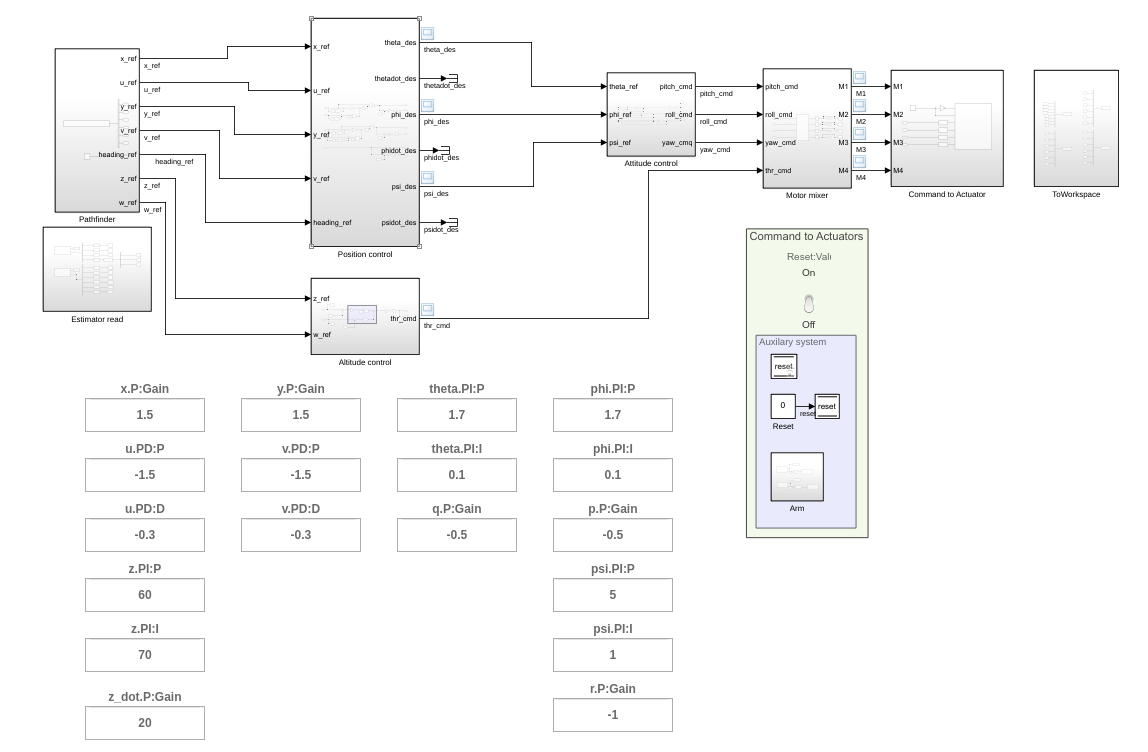
\includegraphics[width=1\textwidth]{DescrizioneAutopilota/Figure/completopid}
	\caption{Modello di controllo completo PID}
\end{figure}

\begin{figure}
	\centering
	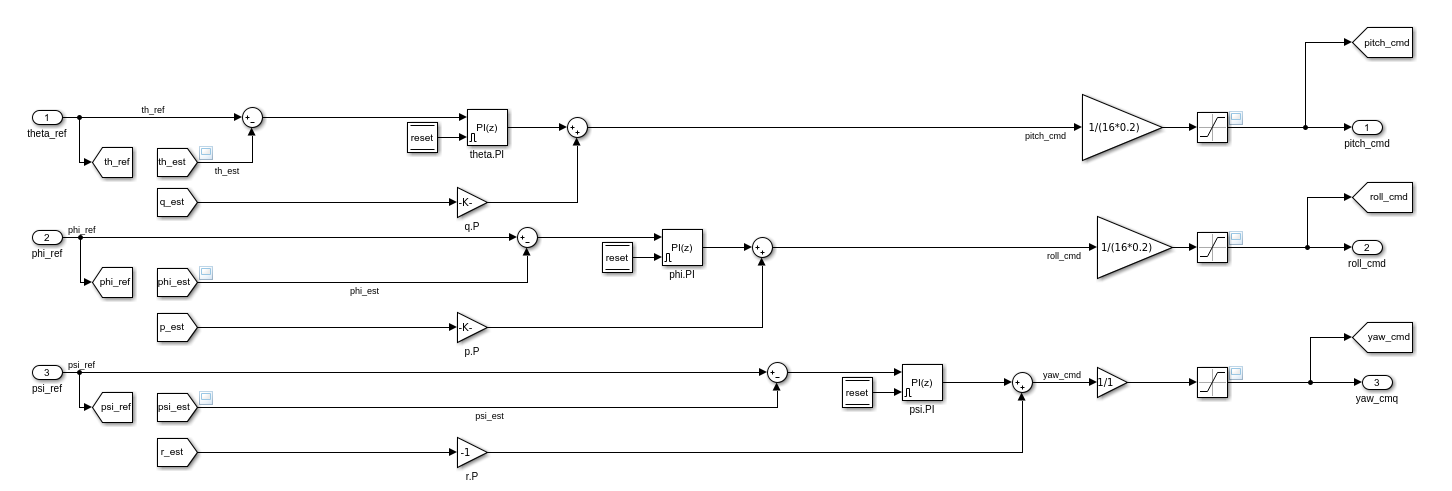
\includegraphics[width=1\textwidth]{DescrizioneAutopilota/Figure/attitudecontrollerpid}
	\caption{Modello di controllo d' assetto PID}
\end{figure}

\begin{figure}
	\centering
	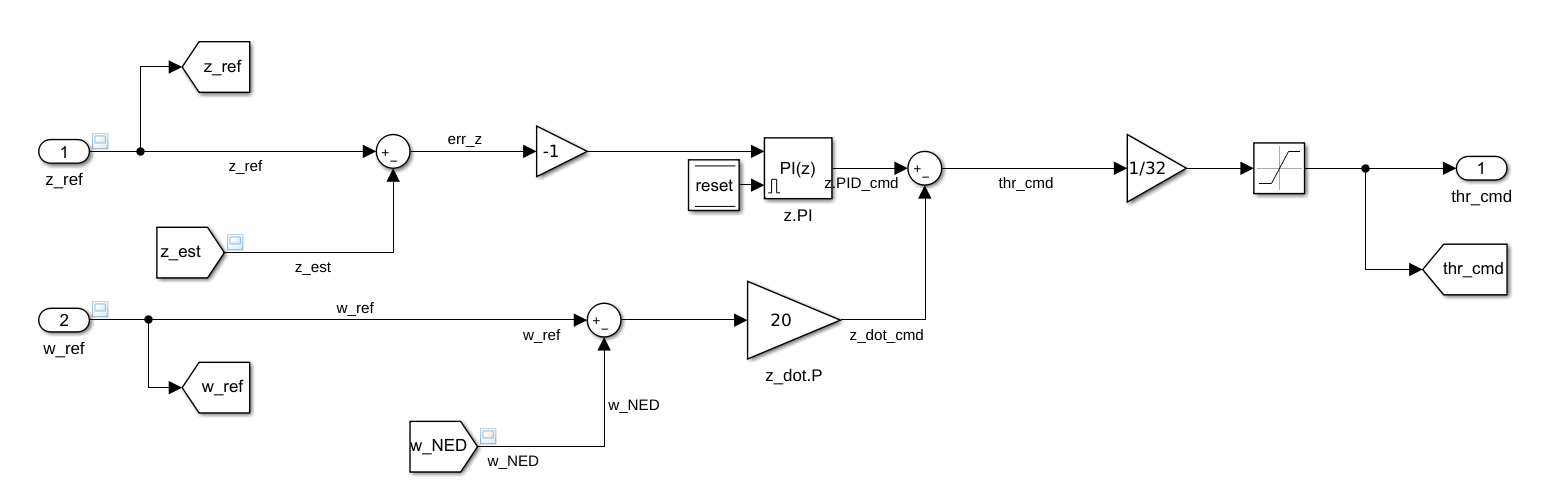
\includegraphics[width=1\textwidth]{DescrizioneAutopilota/Figure/altitudecontrollerpid}
	\caption{Modello di controllo di altitudine PID}
\end{figure}

\begin{figure}
	\centering
	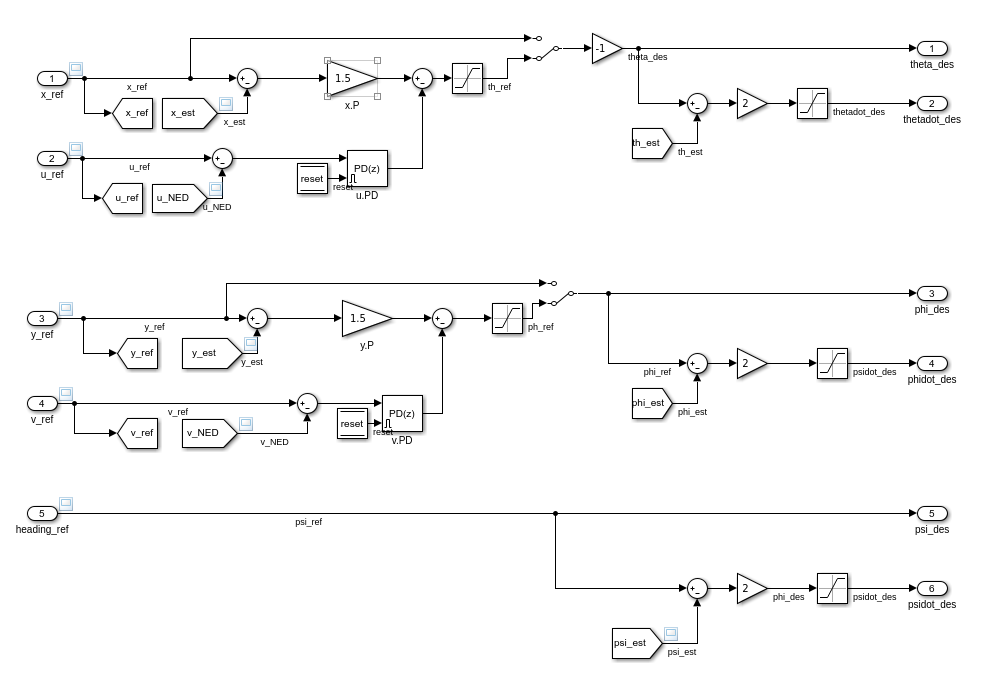
\includegraphics[width=1\textwidth]{DescrizioneAutopilota/Figure/positioncontrollerpid}
	\caption{Modello di controllo di posizione PID}
\end{figure}

\begin{figure}
	\centering
	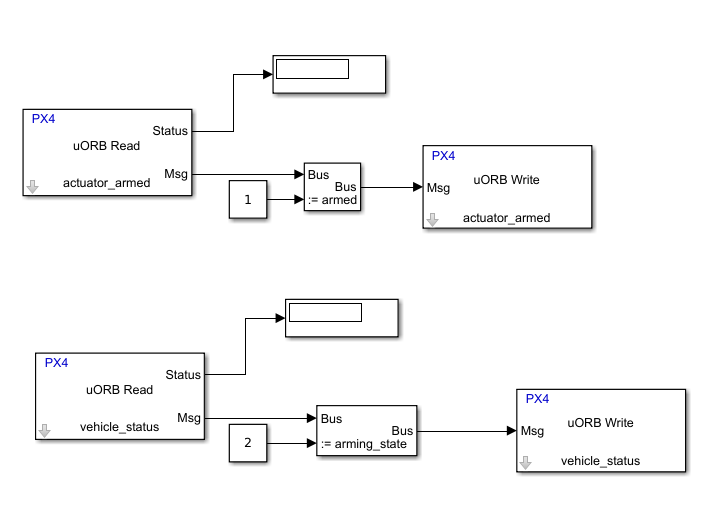
\includegraphics[width=0.5\textwidth]{DescrizioneAutopilota/Figure/armpid}
	\caption{Modello di gestione dei segnali di armamento}
\end{figure}

\todo[inline]{Inserire le tabelle con i parametri}